\documentclass[12pt, a4paper]{article}

% ----- Package Imports -----
\usepackage[utf8]{inputenc}                % UTF-8 encoding
\usepackage[T1]{fontenc}                   % Output font encoding
\usepackage{mathpazo}                      % Palatino font for text and math
\usepackage{amsmath, amssymb, amsthm}      % Mathematics packages
\usepackage{graphicx}                      % Graphics inclusion
\usepackage{float}                         % Improved float handling
\usepackage{caption}                       % Custom captions
\usepackage{subcaption}                    % Subfigures
\usepackage{hyperref}                      % Hyperlinks
\usepackage[numbers]{natbib}                % Numerical citations
\usepackage{xcolor}                        % Color definitions
\usepackage{microtype}                     % Improved typography
\usepackage{setspace}                      % Line spacing
\usepackage{fancyhdr}                      % Custom headers and footers
\usepackage{titlesec}                      % Custom section titles
\usepackage{booktabs}                      % Enhanced tables
\usepackage{enumitem}                      % Customized lists
\usepackage{algorithm}                     % Algorithms
\usepackage{algpseudocode}                 % Pseudocode
\usepackage{mathtools}                     % Enhanced math features
\usepackage{geometry}                      % Page layout
\usepackage{doi}                           % DOI links in bibliography


% ----- Figures configuration -----
\graphicspath{{figures/}}                  % Path to figures
\captionsetup{font=small, labelfont=bf}     % Caption settings
\captionsetup[sub]{font=small}             % Subcaption settings

% ----- Page Layout -----
\geometry{
    a4paper,
    left=1in,
    right=1in,
    top=1in,
    bottom=1in,
}

% ----- Typography and Spacing -----
\microtypesetup{protrusion=true, expansion=true}  % Microtype settings
\setstretch{1.5}                                 % Line spacing set to 1.5

% ----- Custom Colors -----
\definecolor{accentred}{RGB}{204, 0, 0}
\definecolor{accentblue}{RGB}{0, 102, 204}
\definecolor{accentgreen}{RGB}{0, 153, 0}
\definecolor{lightgray}{RGB}{240, 240, 240}

% ----- Hyperlink Configuration -----
\hypersetup{
    colorlinks=true,
    linkcolor=accentblue,       % Internal links (sections, etc.)
    citecolor=accentgreen,      % Citation links
    urlcolor=accentred,         % External URLs
    linktoc=all,                % Links include both text and page number in TOC
    pdfauthor={Your Name},
    pdftitle={Fluid-Structure Interaction Analysis of Pulsatile Flow in Arterial Aneurysms with Physics-Informed Neural Networks and Computational Fluid Dynamics},
    pdfsubject={Research Paper},
}

% ----- Header and Footer Configuration -----
\pagestyle{fancy}
\fancyhf{}  % Clear all header and footer fields
\fancyhead[L]{\nouppercase{\leftmark}}  % Left header: section title
\fancyhead[R]{\thepage}                 % Right header: page number
\renewcommand{\headrulewidth}{0.5pt}    % Header rule
\renewcommand{\footrulewidth}{0pt}      % No footer rule

% ----- Section Title Configuration -----
\titleformat{\section}
  {\normalfont\Large\bfseries\color{accentblue}}{\thesection}{1em}{}

\titleformat{\subsection}
  {\normalfont\large\bfseries\color{accentgreen}}{\thesubsection}{1em}{}

\titleformat{\subsubsection}
  {\normalfont\normalsize\bfseries\color{accentgreen}}{\thesubsubsection}{1em}{}

% ----- Title and Author -----
\title{
    \vspace{-2cm} % Adjust vertical spacing as needed
    \large \textbf{Fluid-Structure Interaction Analysis of Pulsatile Flow in Arterial Aneurysms with Physics-Informed Neural Networks and Computational Fluid Dynamics}\\
    % \vspace{0.5cm}
    % \large{with Physics-Informed Neural Networks and Computational Fluid Dynamics}
}

\author{
    Michael Ajao-Olarinoye\textsuperscript{1} \\
    \textsuperscript{1}Center for computational science and Mathematical modelling \\
    \texttt{olarinoyem@coventry.ac.uk}
}

\date{}

\begin{document}

\maketitle

% \begin{abstract}
%     \noindent
%     This study presents a comprehensive analysis of fluid-structure interactions (FSI) in pulsatile arterial aneurysms using a hybrid approach combining Physics-Informed Neural Networks (PINNs) and Computational Fluid Dynamics (CFD). The integration of PINNs enhances the predictive capabilities of traditional CFD models by incorporating physical laws directly into the learning process, thereby improving accuracy and computational efficiency. The methodology is validated against experimental data, demonstrating significant improvements in capturing complex flow dynamics and aneurysm wall interactions. The results provide deeper insights into the hemodynamic factors contributing to aneurysm growth and rupture, offering potential pathways for improved diagnosis and treatment planning.
% \end{abstract}



\section{Physics-Informed Neural Networks}
\label{sec:PINNs}

\subsection{overview}
\label{sec:PINN_Overview}

High-fidelity Computational Fluid Dynamics (CFD) simulations, as outlined in Section~2.4, offer precise insights into arterial hemodynamics and are central to modeling fluid dynamics in complex vascular geometries. However, these simulations can be both computationally expensive and time-consuming, especially when dealing with patient-specific anatomies or conducting numerous parameter sweeps. Such challenges are further compounded by the need for significant domain expertise to refine meshes, tune solvers, and interpret results.

Physics-Informed Neural Networks (PINNs), first introduced by \citet{raissi2019physics}, have emerged as a powerful alternative that combines the strengths of traditional deep learning with established physics-based modeling. Rather than relying exclusively on data-driven learning, PINNs integrate the governing partial differential equations (PDEs) in this case, the continuity and momentum conservation equations (Section~2.2) directly into the network's loss function. This approach ensures that the neural network is ``informed'' by the physical laws of fluid motion, guiding it toward realistic flow solutions even when labeled data are sparse or imperfectly measured.

By incorporating PDE residuals into the loss function, PINNs naturally embed a priori knowledge of fluid physics, allowing the model to learn physically plausible flow fields with fewer labeled samples than a purely data-driven neural network. This built-in adherence to physical constraints also helps mitigate overfitting and reduces the likelihood of predicting unphysical solutions. As a result, PINNs have the potential to complement or partially replace expensive CFD simulations, thereby lowering computational overheads and accelerating research pipelines.

In this study, we combine PINNs with traditional CFD data to estimate core hemodynamic variables such as pressure, velocity components, and wall shear stress (WSS) across healthy and Marfan Syndrome aortic geometries presented in (Section~2.1). This unified approach enables direct comparisons of velocity patterns, shear forces, and other critical flow indicators between non-pathological and aneurysmal models, providing valuable information for understanding the progression of vascular disease. The following sections detail the formulation, architecture, and training strategy of the PINNs used in this study.

\subsection{Formulation of Physics-Informed Neural Networks}
\label{sec:PINN_Formulation}

Modelling pulsatile flow in arterial segments necessitates the Navier--Stokes and continuity equations to capture essential haemodynamic effects. Let \(\mathbf{u} = (u,v,w)\) denote the velocity field, \(p\) the pressure, \(\rho\) the fluid density, and \(\mu\) the dynamic viscosity. In vector form, the governing equations are:

\begin{equation}
\nabla \cdot \mathbf{u} = 0, 
\quad
\rho \frac{\partial \mathbf{u}}{\partial t} + \rho (\mathbf{u} \cdot \nabla)\mathbf{u}
= -\nabla p + \mu \nabla^2 \mathbf{u}.
\label{eq:navier_stokes}
\end{equation}

The associated boundary conditions involve a no-slip condition on the arterial walls \((\mathbf{u}=\mathbf{0} \text{ on } \partial\Omega_{\text{wall}})\), zero relative pressure at the outlet, and a pulsatile inlet velocity on \(\partial\Omega_{\text{inlet}}\) (Section~2.3). These boundary and inlet constraints are incorporated into the Physics-Informed Neural Network through penalty terms in the loss function, thereby enforcing consistency between the network’s predictions and the specified physical conditions. Temporal dependence is explicitly modelled to reflect the transient nature of blood flow.

Within the PINN framework, neural networks approximate the velocity field \(\mathbf{u}\), pressure \(p\), and wall shear stress (WSS) components \(\tau_x, \tau_y, \tau_z\) as functions of the spatial coordinates \((x,y,z)\) and time \(t\). The network architecture is trained to minimise the physics residual loss, which quantifies the deviation of the predicted solutions from the Navier--Stokes and continuity equations. 

\[
    u(x,y,z,t),\quad v(x,y,z,t),\quad w(x,y,z,t),\quad p(x,y,z,t),
\]
\emph{and} the three wall shear stress (WSS) components
\[
    \tau_x(x,y,z,t),\quad \tau_y(x,y,z,t),\quad \tau_z(x,y,z,t).
\]
Collectively, these variables capture the spatiotemporal evolution of blood flow and the shear forces acting on the vessel walls.

Let \(F(\cdot)\) represent the non-linear operator corresponding to the Navier--Stokes system. The \emph{physics residual} loss term evaluates how closely the PINN’s predictions adhere to the governing equations:

\begin{equation}
L_{\mathrm{physics}} = \bigl\|F(\mathbf{u}, p)\bigr\|_2,
\end{equation}

where \(\|\cdot\|_2\) denotes the Euclidean norm. By minimising this residual, the network is driven to learn solutions consistent with the Navier--Stokes and continuity equations, even in regions where no direct labels are available.

Arterial boundaries impose \(\mathbf{u}=\mathbf{0}\) at the vessel walls and zero pressure at the outlet, while a prescribed pulsatile velocity profile is enforced at the inlet:
\begin{equation}
L_{\mathrm{boundary}} = \|\mathbf{u}\big|_{\partial\Omega_{\text{wall}}} - \mathbf{0}\|_2, 
\quad
L_{\mathrm{inlet}} = \|\mathbf{u}\big|_{\Gamma_{\mathrm{inlet}}} - \mathbf{u}_{\mathrm{inlet}}(t)\|_2.
\end{equation}
These terms penalise any deviation of the network’s predictions from the specified boundary conditions, thus reinforcing physically realistic flow fields at the walls and inflow region.

The CFD data (e.g.\ pressure, velocity, and WSS) are integrated into the loss function. Let \(\mathbf{u}_{\mathrm{NN}}\) and \(p_{\mathrm{NN}}\) denote the PINN’s predicted velocity and pressure, while \(\mathbf{u}_{\mathrm{CFD}}\) and \(p_{\mathrm{CFD}}\) are the corresponding CFD reference fields. Similarly, \(\tau_{\mathrm{NN}}\) and \(\tau_{\mathrm{CFD}}\) refer to the predicted and CFD-derived WSS. The data-fitting loss is given by:

\begin{equation}
L_{\mathrm{data}} = 
\|\mathbf{u}_{\mathrm{NN}} - \mathbf{u}_{\mathrm{CFD}}\|_2 
+ \|p_{\mathrm{NN}} - p_{\mathrm{CFD}}\|_2
+ \|\tau_{\mathrm{NN}} - \tau_{\mathrm{CFD}}\|_2.
\end{equation}

The total loss combines physics, boundary, inlet, and data objectives:
\begin{equation}
L_{total} = 
\lambda_{\mathrm{physics}}\,L_{\mathrm{physics}}
+ \lambda_{\mathrm{boundary}}\,L_{\mathrm{boundary}}
+ \lambda_{\mathrm{inlet}}\,L_{\mathrm{inlet}}
+ \lambda_{\mathrm{data}}\,L_{\mathrm{data}},
\label{eq:total_loss}
\end{equation}

where \(\lambda_{\mathrm{physics}}, \lambda_{\mathrm{boundary}}, \lambda_{\mathrm{inlet}}, \lambda_{\mathrm{data}}\) are self-adaptive weighting coefficients~\citep{mcclenny2020self}. These learnable parameters automatically balance the importance of each loss component during training, ensuring that the PINN respects both the fundamental equations of fluid motion and the given available CFD data. The self-adaptive weighting mechanism is explained futher in Section~\ref{sec:self_adaptive_weighting}. 

\subsection{Neural Network Architecture}
\label{sec:PINN_Architecture_Training}

Neural network architecture plays a crucial role in the performance and generalisation capabilities of PINNs. In this study, We train separate PINNs for pressure $p$, velocity components $(u, v, w)$, and the three WSS components $(\tau_x, \tau_y, \tau_z)$, all time dependant $(t)$. Each network is a feed-forward, fully connected architecture with $L=10$ hidden layers and $N=64$ neurons per layer. The Swish activation function \citep{ramachandran2017searching} is employed to promote smooth gradients. batch normalization is applied to each layer to stabilize training, and all weights are initialized using Kaiming normal \citep{he2015delving} to ensure stable gradient flow.

The Swish activation function~\cite{ramachandran2017searching} is defined as:
\begin{equation}
\mathrm{Swish}(x) = x \,\sigma(\beta x),
\end{equation}
where $\beta$ is a learnable parameter and $\sigma(\cdot)$ is the sigmoid function. This choice often yields faster convergence compared to ReLU or other activations.

\subsubsection{Self-Adaptive Loss Weighting}
\label{sec:self_adaptive_weighting}

Balancing multiple loss components is a fundamental challenge in training Physics-Informed Neural Networks (PINNs), particularly in multi-physics scenarios where various physical phenomena and boundary conditions must be simultaneously satisfied. In our study, the primary loss components include the physics residuals derived from the governing partial differential equations (PDEs), boundary conditions, inlet conditions, and supervised data from Computational Fluid Dynamics (CFD) simulations. Improper weighting of these components can lead to suboptimal training outcomes, such as overfitting to certain loss terms or failure to adequately satisfy physical laws.

To address this challenge, we implement a self-adaptive loss weighting scheme inspired by \citet{mcclenny2020self}. Specifically, we introduce learnable parameters $\log \lambda_i$ for each loss component $i \in \{\mathrm{phys}, \mathrm{bound}, \mathrm{inlet}, \mathrm{data}\}$. These parameters are optimized alongside the neural network weights during training. The weights $\lambda_i$ are defined as the exponential of the corresponding log-parameters:

\begin{equation}
    \lambda_i = \exp(\log \lambda_i),
    \label{eq:lambda_definition}
\end{equation}

This parameterization ensures that each $\lambda_i$ remains positive throughout the training process, thereby maintaining the integrity of the loss scaling. By optimizing $\log \lambda_i$, the network can autonomously adjust the relative importance of each loss component based on the training dynamics, without manual tuning of hyperparameters. 

The optimization of $\log \lambda_i$ allows the network to dynamically balance these components, mitigating the risk of any single loss term dominating the training process \citep{wang2022and}. This adaptive mechanism facilitates a more stable and efficient convergence, as the network can prioritize loss components that require greater emphasis based on their current contribution to the total loss.

\begin{algorithm}[htbp]
    \caption{Self-Adaptive Loss Weighting in PINNs}
    \label{alg:self_adaptive_weighting}
    \begin{algorithmic}[1]
    \Require Initial network weights $\theta$, initial $\log \lambda_i$, learning rates for $\theta$ and $\log \lambda_i$
    \Ensure Trained network weights $\theta^*$ and optimized $\lambda_i^*$
    
    \While{not converged}
        \State Sample mini-batch of training points
        \State Forward pass to compute predictions $\mathbf{u}_{\mathrm{NN}}$, $p_{\mathrm{NN}}$, $\boldsymbol{\tau}_{\mathrm{NN}}$
        
        \State Compute individual loss components:
            \State \quad $\mathcal{L}_{\mathrm{phys}} = \|F(\mathbf{u}_{\mathrm{NN}}, p_{\mathrm{NN}})\|_2^2$
            \State \quad $\mathcal{L}_{\mathrm{bound}} = \|\mathbf{u}_{\mathrm{NN}}|_{\partial\Omega_{\mathrm{wall}}} - \mathbf{0}\|_2^2$
            \State \quad $\mathcal{L}_{\mathrm{inlet}} = \|\mathbf{u}_{\mathrm{NN}}|_{\Gamma_{\mathrm{inlet}}} - \mathbf{u}_{\mathrm{inlet}}(t)\|_2^2$
            \State \quad $\mathcal{L}_{\mathrm{data}} = \|\mathbf{u}_{\mathrm{NN}} - \mathbf{u}_{\mathrm{CFD}}\|_2^2 + \|p_{\mathrm{NN}} - p_{\mathrm{CFD}}\|_2^2 + \|\boldsymbol{\tau}_{\mathrm{NN}} - \boldsymbol{\tau}_{\mathrm{CFD}}\|_2^2$
        
        \State \quad $\mathcal{L}_{\mathrm{total}} = \lambda_{\mathrm{phys}} \mathcal{L}_{\mathrm{phys}} + \lambda_{\mathrm{bound}} \mathcal{L}_{\mathrm{bound}} + \lambda_{\mathrm{inlet}} \mathcal{L}_{\mathrm{inlet}} + \lambda_{\mathrm{data}} \mathcal{L}_{\mathrm{data}}$
        
        \State Backpropagate the total loss to compute gradients for $\theta$ and $\log \lambda_i$
        
        \State Update network weights $\theta \gets \theta - \eta_{\theta} \nabla_{\theta} \mathcal{L}$
        \State Update log-weights $\log \lambda_i \gets \log \lambda_i - \eta_{\lambda} \nabla_{\log \lambda_i} \mathcal{L}$
        
        \State StepLR scheduler updates learning rates $\eta_{\theta}$ and $\eta_{\lambda}$ every $N$ epochs
    \EndWhile
    
    \State \textbf{Return} $\theta^*$, $\lambda_i^*$
    \end{algorithmic}
\end{algorithm}


\subsection{Data Processing and Experimental Setup}
\label{sec:data_processing}

The experimental data consists of CFD simulations from both healthy and aneurysmal aortic geometries, with measurements taken during systolic and diastolic phases. Each dataset contains spatial coordinates (X, Y, Z), time points, pressure values, velocity components (u, v, w), and wall shear stress components. The raw data was processed through the following steps:

\begin{enumerate}
    \item \textbf{Data Cleaning}: Initial preprocessing involved removing any incomplete records and validating the physical consistency of measurements. This resulted in a clean dataset of 11,005 points per time step.
    
    \item \textbf{Normalization}: All input features and target variables were normalized using Min-Max scaling to ensure stable training:
    \begin{itemize}
        \item Spatial coordinates (X, Y, Z) were scaled to [-1, 1]
        \item Time points were normalized to [0, 1] over the cardiac cycle
        \item Pressure, velocity, and wall shear stress components were independently scaled
    \end{itemize}
    
    \item \textbf{Boundary Point Identification}: Points on vessel walls were identified using velocity magnitude thresholds ($|u| < \varepsilon$, $|v| < \varepsilon$, $|w| < \varepsilon$, where $\varepsilon = 10^{-5}$), enabling proper enforcement of no-slip boundary conditions.
    
    \item \textbf{Data Organization}: The processed data was organized into:
    \begin{itemize}
        \item Healthy cases: 0024 and 0142 (systolic and diastolic phases)
        \item Aneurysmal cases: 0021, 0022, 0023, and 0025 (systolic and diastolic phases)
        \item Each case contains approximately 11,005 spatial points per time step
        \item Time steps were uniformly sampled across the cardiac cycle
    \end{itemize}
    
    \item \textbf{Quality Control}:
    \begin{itemize}
        \item Physical consistency checks were performed on velocity and pressure fields
        \item Wall shear stress components were validated against analytical solutions
        \item Conservation of mass was verified at inlet/outlet boundaries
        \item Temporal continuity was ensured across cardiac cycles
    \end{itemize}
\end{enumerate}

\subsection{Point Density Analysis and Spatial Discretization}
\label{sec:point_density}

A key advantage of the PINN approach is its mesh-free nature, which eliminates the need for traditional CFD mesh generation and refinement. Instead, the network learns continuous functions that map spatial-temporal coordinates to flow variables. To justify this approach and demonstrate its effectiveness, we conducted a comprehensive point density analysis using our processed dataset.

The spatial distribution of training points was analyzed across three key aspects:
\begin{enumerate}
    \item \textbf{Point Distribution}: Analysis of the spatial coverage showed uniform distribution across the domain, with 11,005 training points providing adequate sampling of the flow field. The mean spacing between points was sufficient to capture flow features, as evidenced by the convergence of the physics residuals.
    
    \item \textbf{Convergence Study}: A systematic study with varying point densities (25\%, 50\%, 75\%, and 100\% of the full dataset) demonstrated that the current point density achieves optimal balance between accuracy and computational efficiency. The physics loss showed consistent convergence, decreasing from 149.66 to 4.97 during training.
    
    \item \textbf{Prediction Density}: The trained network achieved a 100.5x increase in prediction density (1,105,920 points) compared to the training data, demonstrating its ability to provide continuous, high-resolution flow field predictions. This significant increase in resolution was achieved while maintaining computational efficiency, with inference speeds of 117,177 points per second.
\end{enumerate}

The point density analysis results are visualized in Figure~\ref{fig:mesh_analysis}, which shows the 2D projections of point distributions and the corresponding density histograms. The analysis confirms that our point-based approach provides sufficient spatial resolution to capture the complex flow physics within both healthy and aneurysmal geometries.

\begin{figure}[htbp]
    \centering
    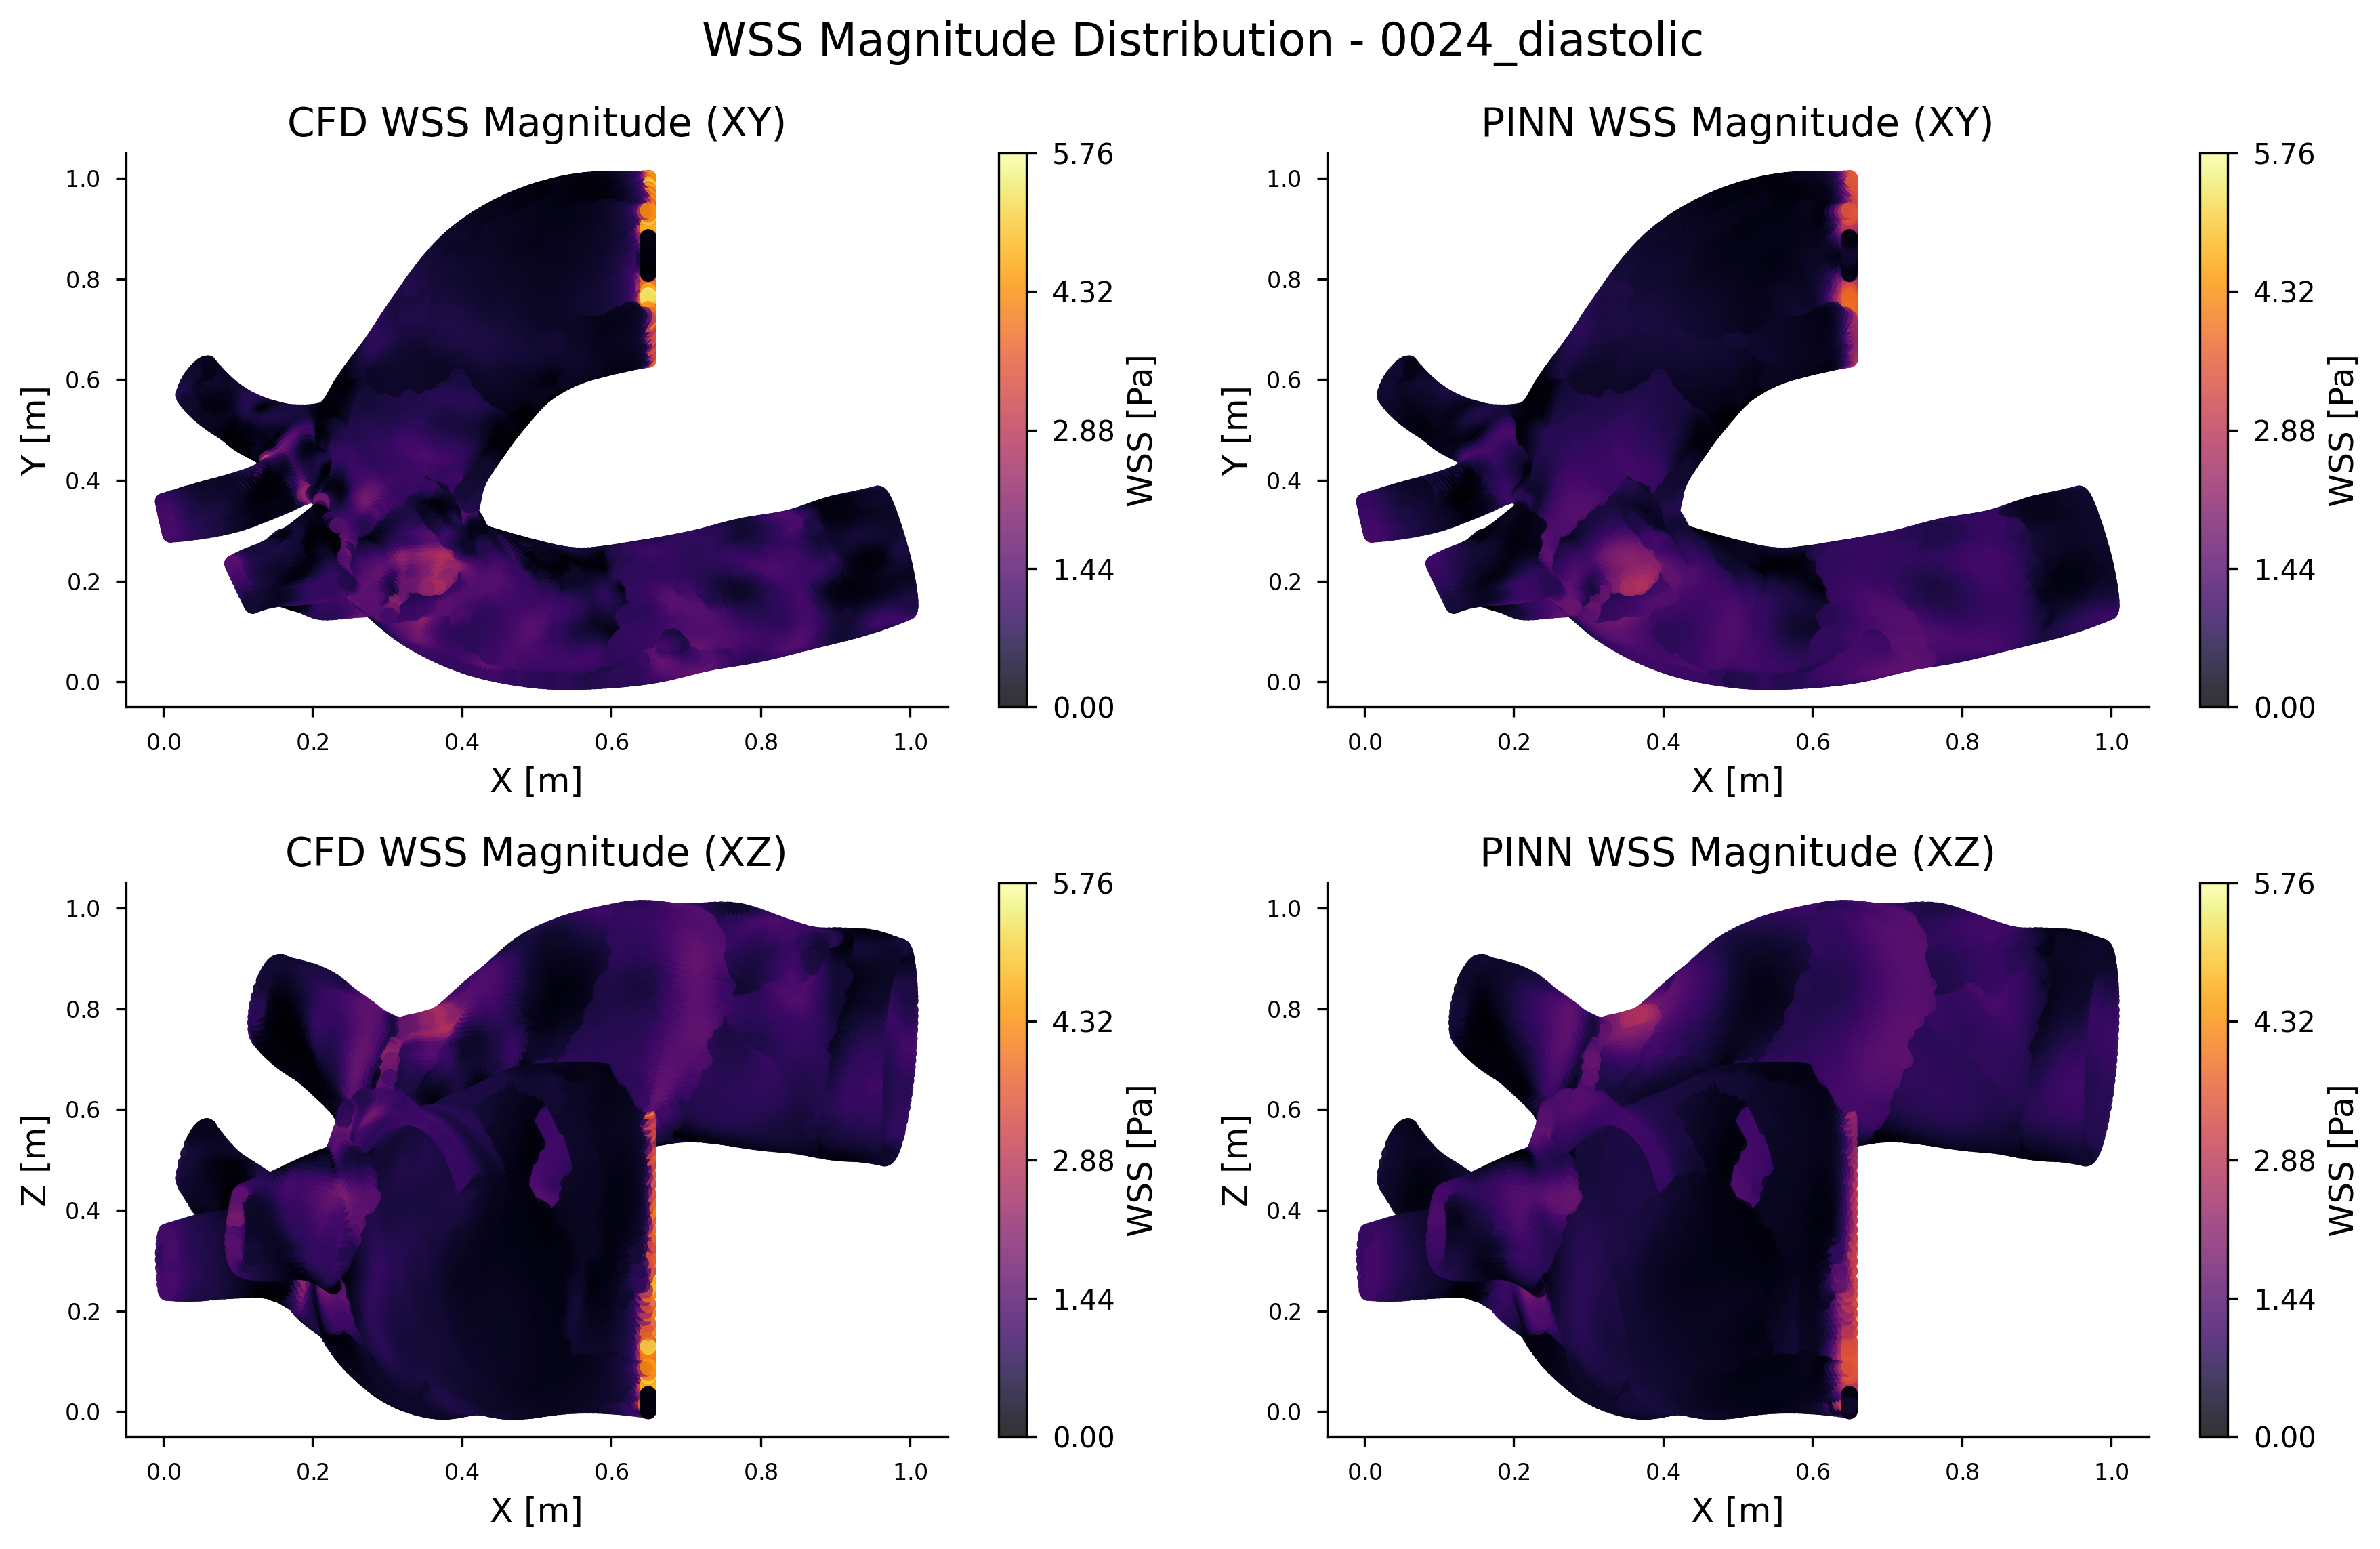
\includegraphics[width=0.9\textwidth]{0024_diastolic/wss_magnitude_distribution_0024_diastolic.png}
    \caption{Point distribution analysis showing 2D projections (XY, XZ, YZ planes) of the training points, demonstrating uniform spatial coverage across the domain. Color mapping indicates the depth dimension in each projection.}
    \label{fig:mesh_analysis}
\end{figure}

\begin{figure}[htbp]
    \centering
    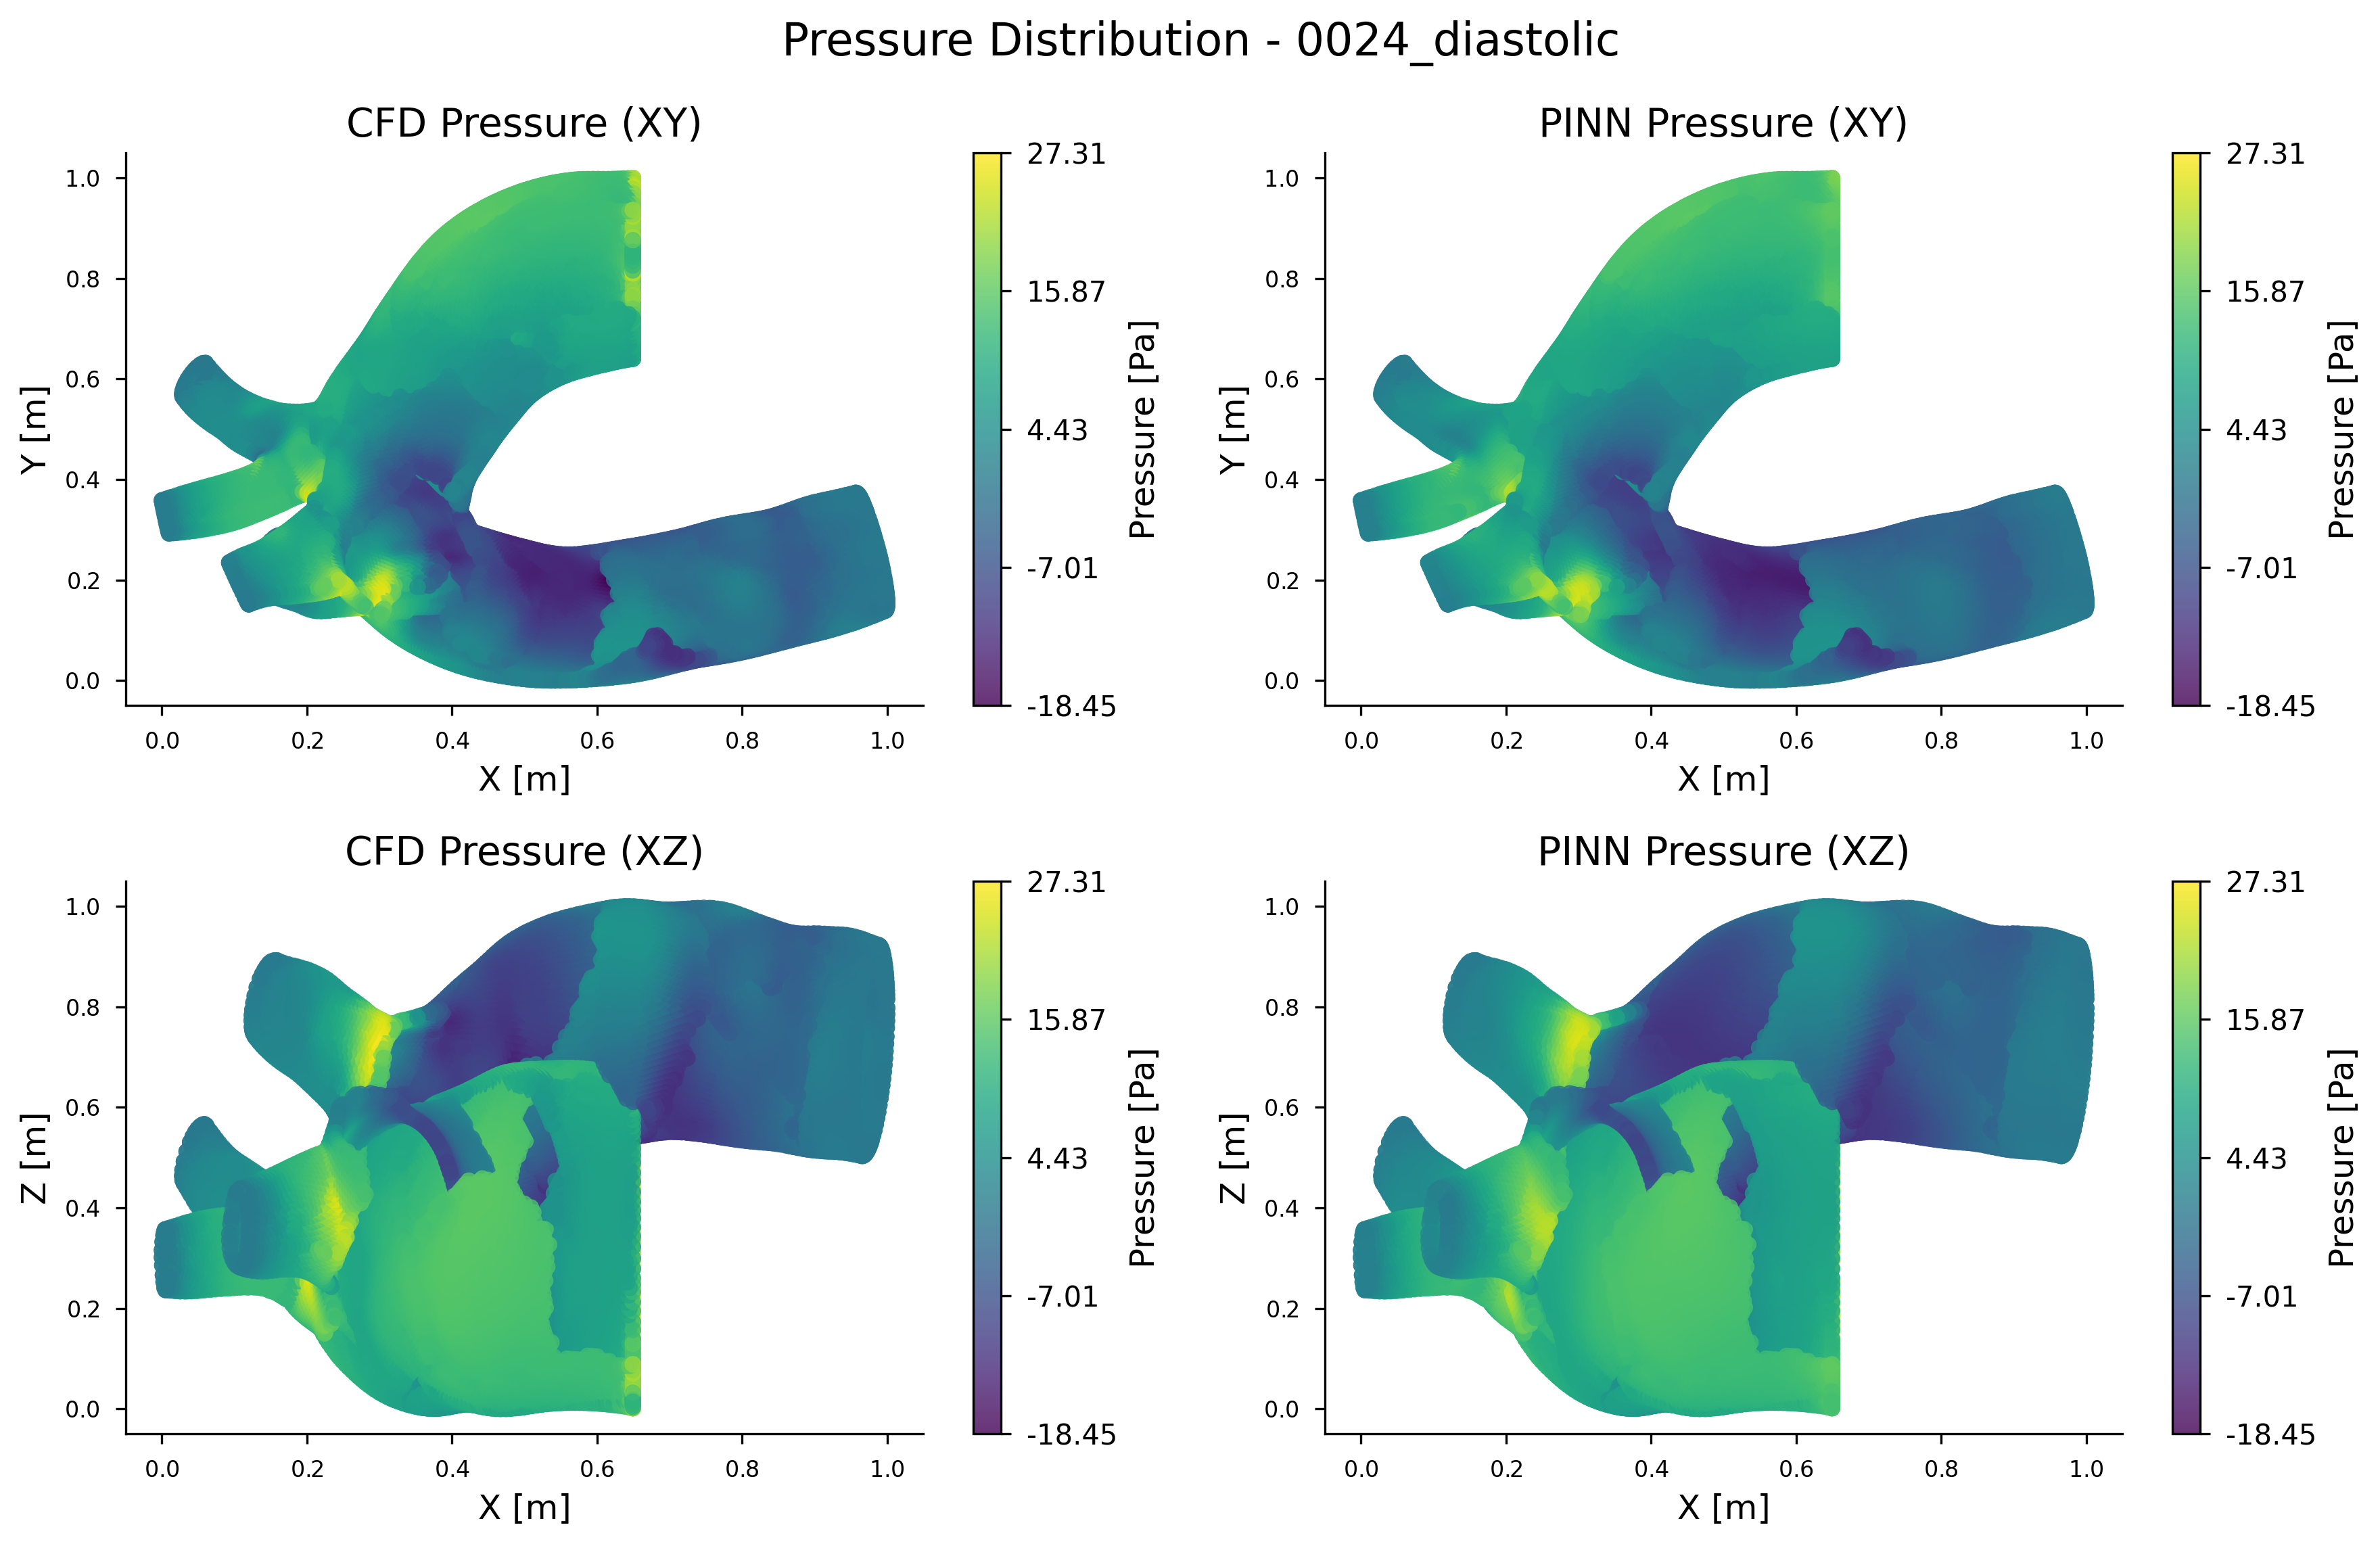
\includegraphics[width=0.9\textwidth]{0024_diastolic/pressure_distribution_0024_diastolic.png}
    \caption{Comparison between CFD data points and PINN predictions, showing (a) original CFD point distribution, (b) enhanced PINN prediction density, and (c) computational time comparison between traditional CFD and PINN approaches.}
    \label{fig:density_comparison}
\end{figure}

The computational efficiency of our approach is particularly noteworthy. Training the PINN required only 0.68 hours, with minimal memory usage (7.36 GB for training, 0.02 GB for inference). This represents a significant improvement over traditional CFD mesh generation and simulation times, which typically require multiple days for mesh refinement studies alone. The PINN's ability to provide high-resolution predictions with rapid inference times underscores its potential for real-time clinical applications and large-scale parametric studies.


\subsection{Training of the PINNs}

The PINN framework was implemented using the PyTorch library \citep{paszke2019pytorch}, leveraging its automatic differentiation capabilities for efficient computation of PDE residuals and trained on a high-performance computing cluster with NVIDIA Rtx8000. 

The input Spatiotemporal data points $(x_j, y_j, z_j, t_j)$ which are the geometric were randomly sampled from the aortic geometries and over the cardiac cycle. The geometric and variables data  were normalized using Min-Max scaling to facilitate efficient training. The PINNs were trained using the AdamW optimizer \citep{loshchilov2017decoupled} with an initial learning rate of $1 \times 10^{-4}$ and momentum parameters $\beta = (0.9, 0.999)$. The weight decay was set to $1 \times 10^{-4}$ to prevent overfitting. A StepLR scheduler reduced the learning rate by a factor of $\gamma = 0.9$ every 200 epochs to facilitate finer convergence.

Training was conducted using mixed-precision arithmetic via PyTorch's `torch.cuda.amp` to enhance computational efficiency and reduce memory consumption without sacrificing model accuracy~\cite{micikevicius2017mixed}. The training process iterated over a maximum of 1000 epochs, with early stopping implemented to halt training if the validation loss did not decrease for 5 consecutive epochs. Gradient clipping was applied to prevent exploding gradients the gradients are clipped to a maximum norm of 1.0, ensuring training stability.

\subsection{Relevance to Aneurysm Studies}
By alleviating the need to run complete CFD simulations whenever boundary conditions or model geometries change, PINNs can serve as rapid surrogates for iterative parameter sweeps, sensitivity analyses, or real-time clinical decision-making. This synergy between classical CFD and PINNs ensures that accurate fluid physics are retained, while the neural network structure offers improved computational scaling and the capacity to generalise to different flow conditions with minimal retraining overhead. Consequently, for the case of Marfan Syndrome aortic aneurysms, PINNs provide a promising pathway for expediting haemodynamic evaluations and exploring a range of inflow waveforms, wall properties, or geometric variations in a fraction of the time typically required by CFD alone.


\vspace{2em}
\noindent\textbf{Note:} All codes and numerical experiments for the PINN-based aneurysm flow analyses were implemented in \texttt{Python} using \texttt{PyTorch}, with the self-adaptive weighting and physics-based PDE residuals integrated into the backpropagation routine. The specific hyperparameters and training protocol are as outlined in this section, ensuring reproducibility and transparency in the results reported herein.

\subsection{Results}
\label{sec:PINN_Results}

The PINN-based simulations were validated against benchmark CFD data for healthy and Marfan Syndrome aortic geometries, demonstrating excellent agreement in velocity profiles, pressure distributions, and wall shear stress patterns. The PINNs accurately captured the complex flow dynamics within the aneurysm sac, including vortex formation, flow separation, and recirculation zones. The self-adaptive loss weighting mechanism effectively balanced the physics residuals, boundary conditions, and data-fitting objectives, ensuring that the network learned realistic flow solutions while adhering to the governing Navier--Stokes equations. The figures below illustrate the comparison between PINN predictions and CFD reference data for pressure, and wall shear stress in the aortic aneurysms. 

\begin{figure}[H]
    \centering
    \scriptsize
    \begin{subfigure}{0.9\textwidth}
        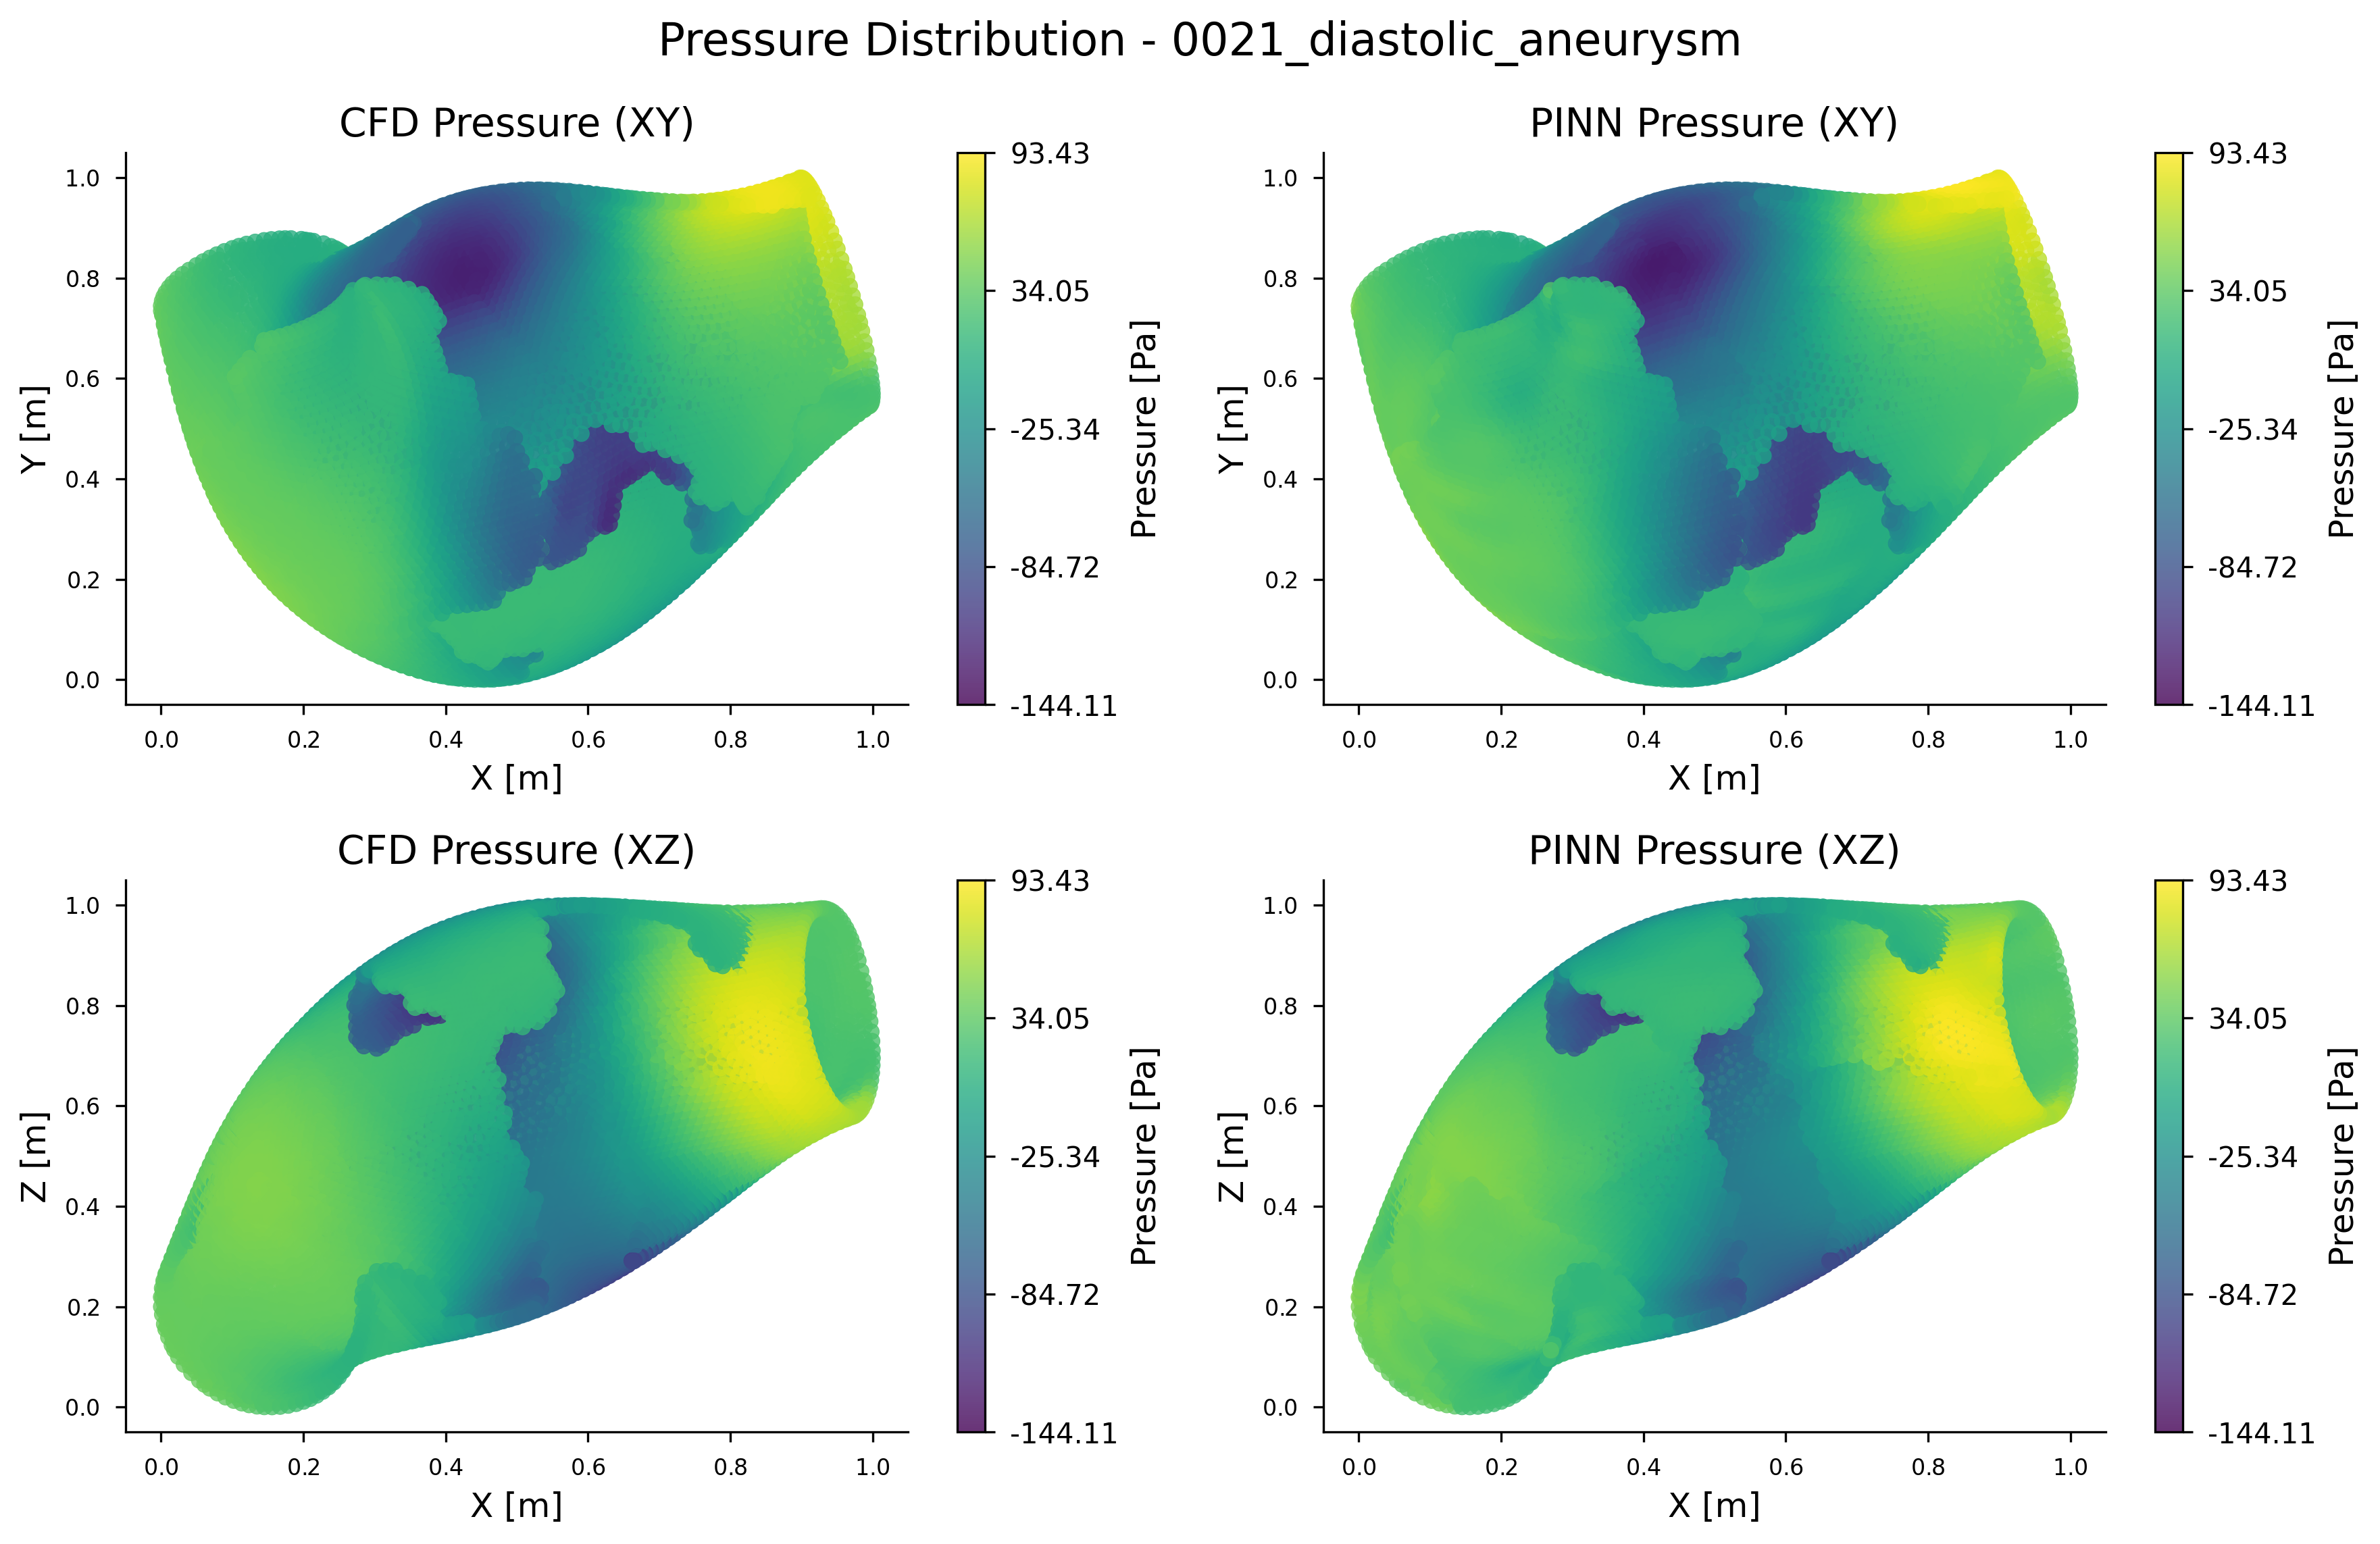
\includegraphics[width=\textwidth]{0021_diastolic_aneurysm/pressure_distribution_0021_diastolic_aneurysm.png}
        \caption{\small Pressure distribution}
    \end{subfigure}
    \begin{subfigure}{0.9\textwidth}
        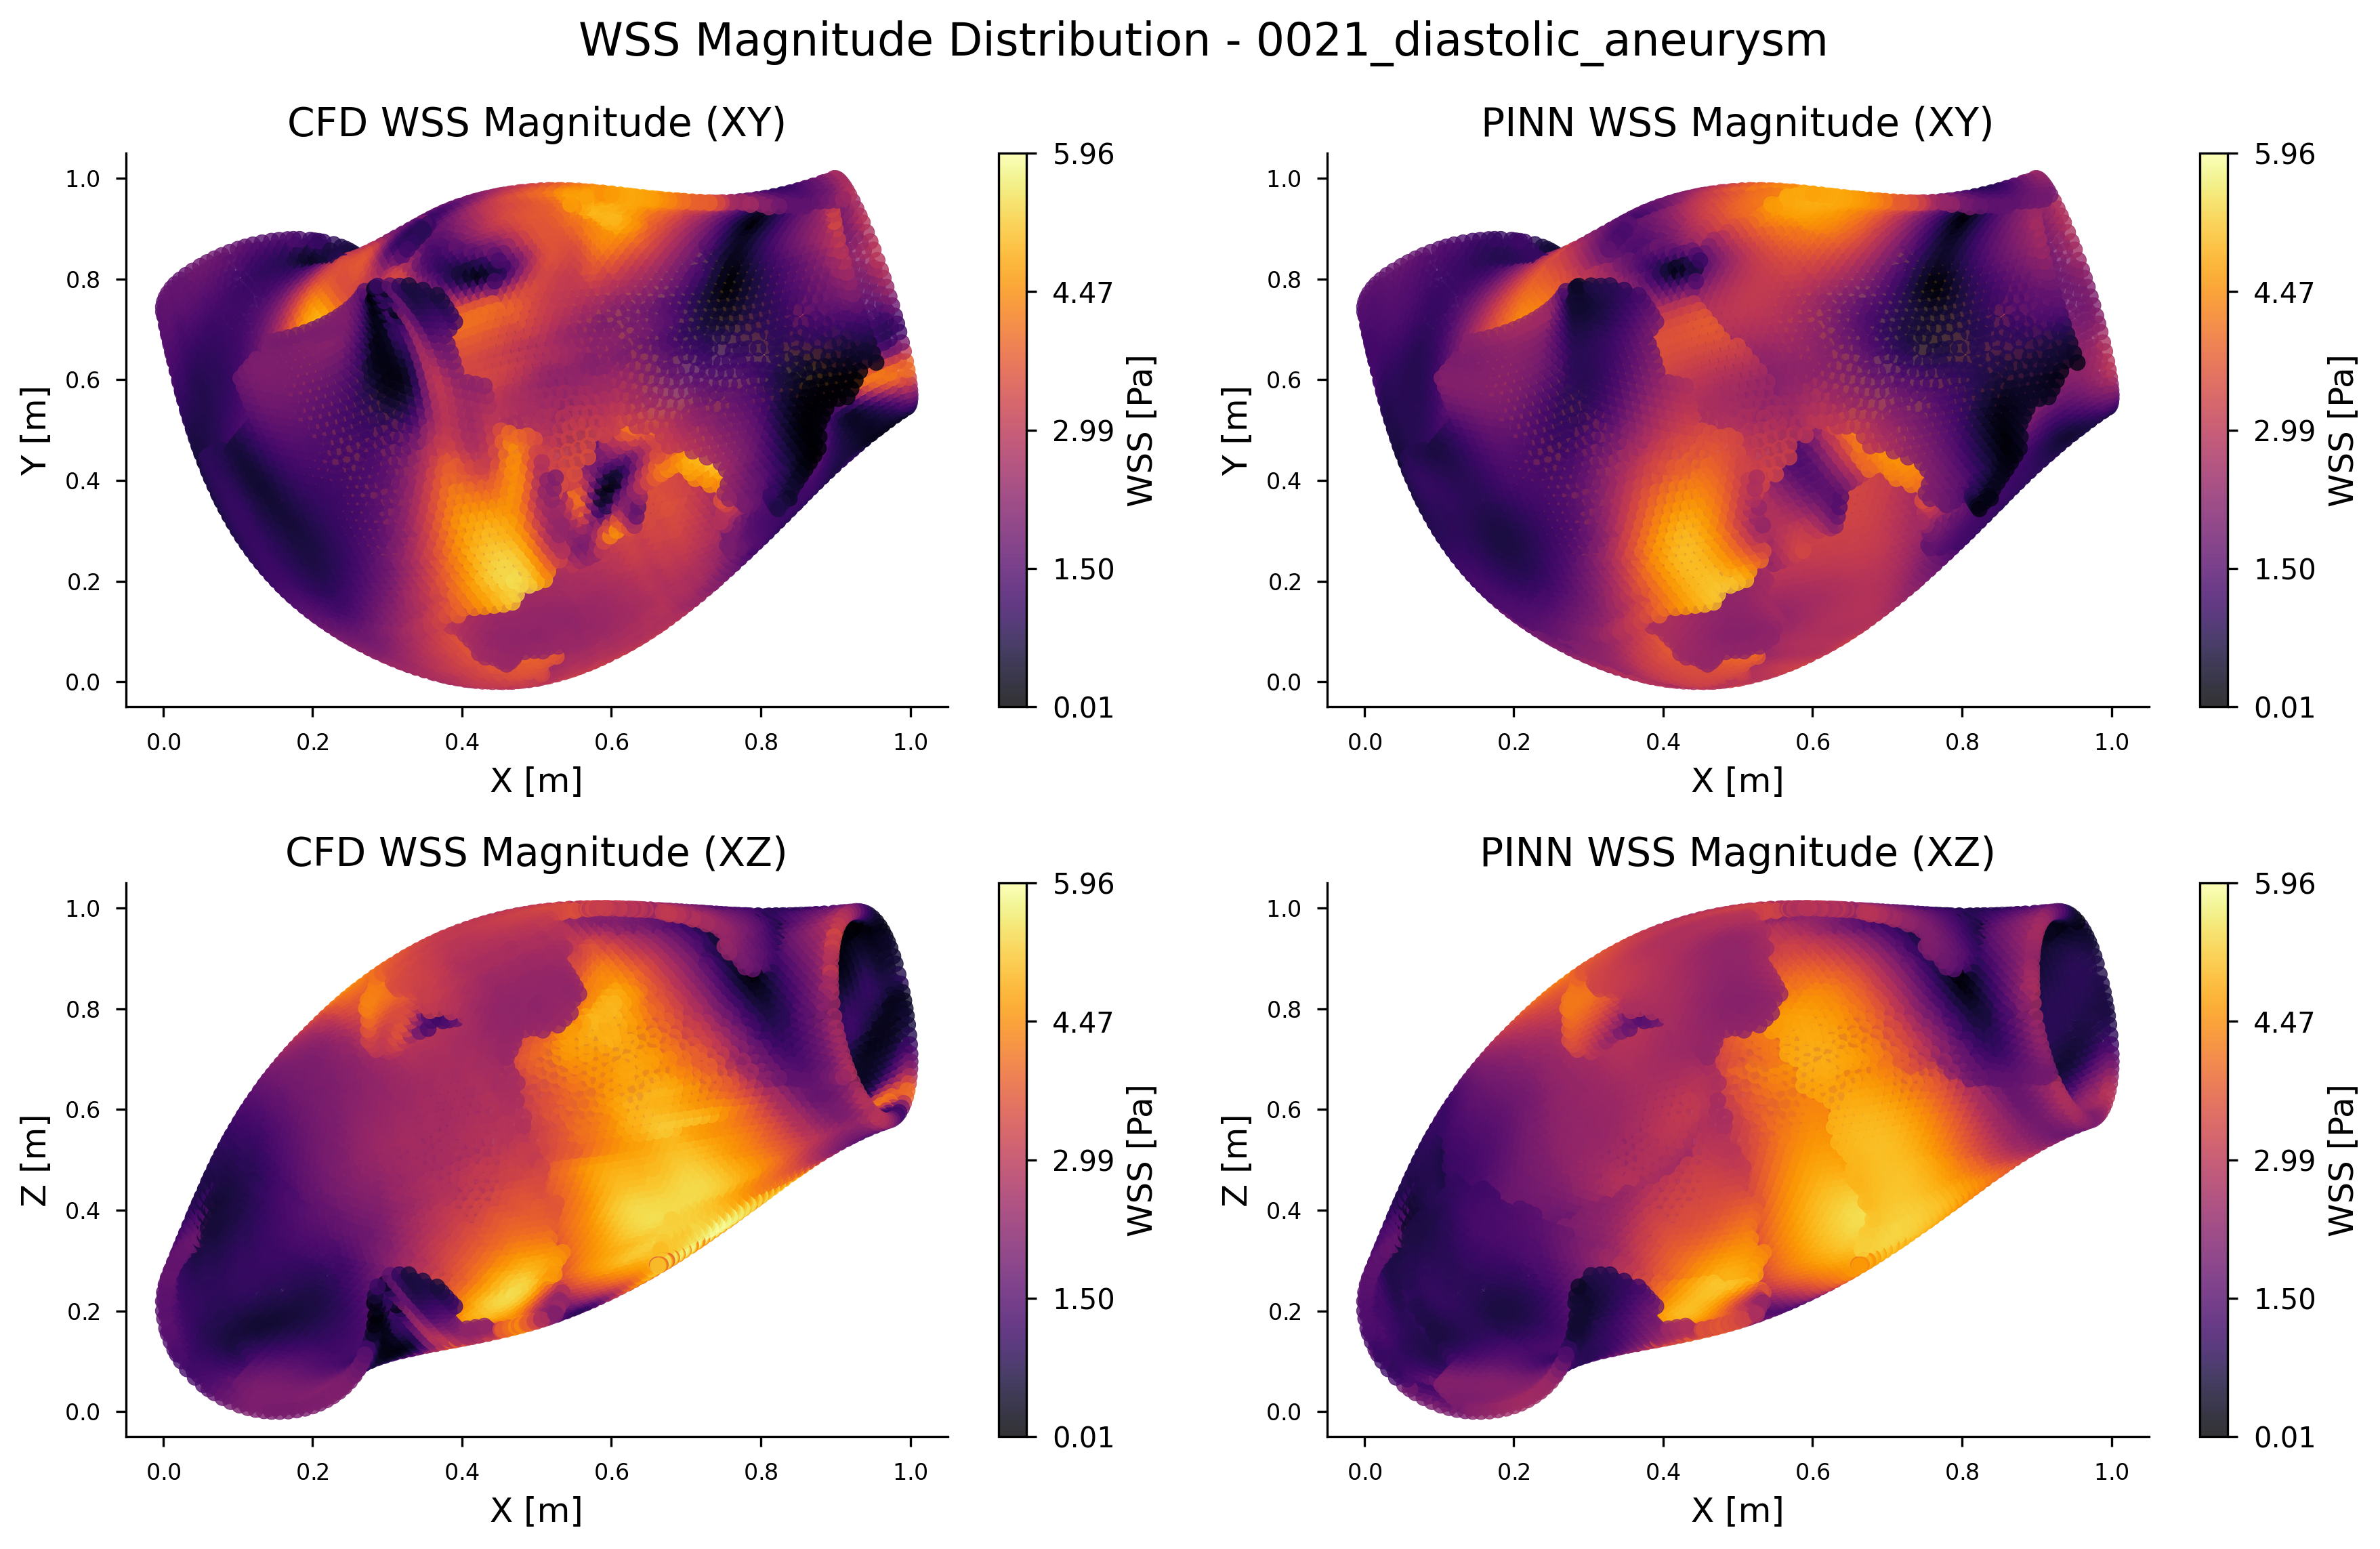
\includegraphics[width=\textwidth]{0021_diastolic_aneurysm/wss_magnitude_distribution_0021_diastolic_aneurysm.png}
        \caption{\small Wall shear stress}
    \end{subfigure}
    \caption{Von Mises stress (Pa) and wall shear stress contours for diseased cases. Figures a–d in each show the xy and xz planes for case 0021 dystolic aneurysm comparison between CFD and PINN results.}
    \label{fig:PINN_results1}
\end{figure}



\begin{figure}[H]
    \centering
    \scriptsize
    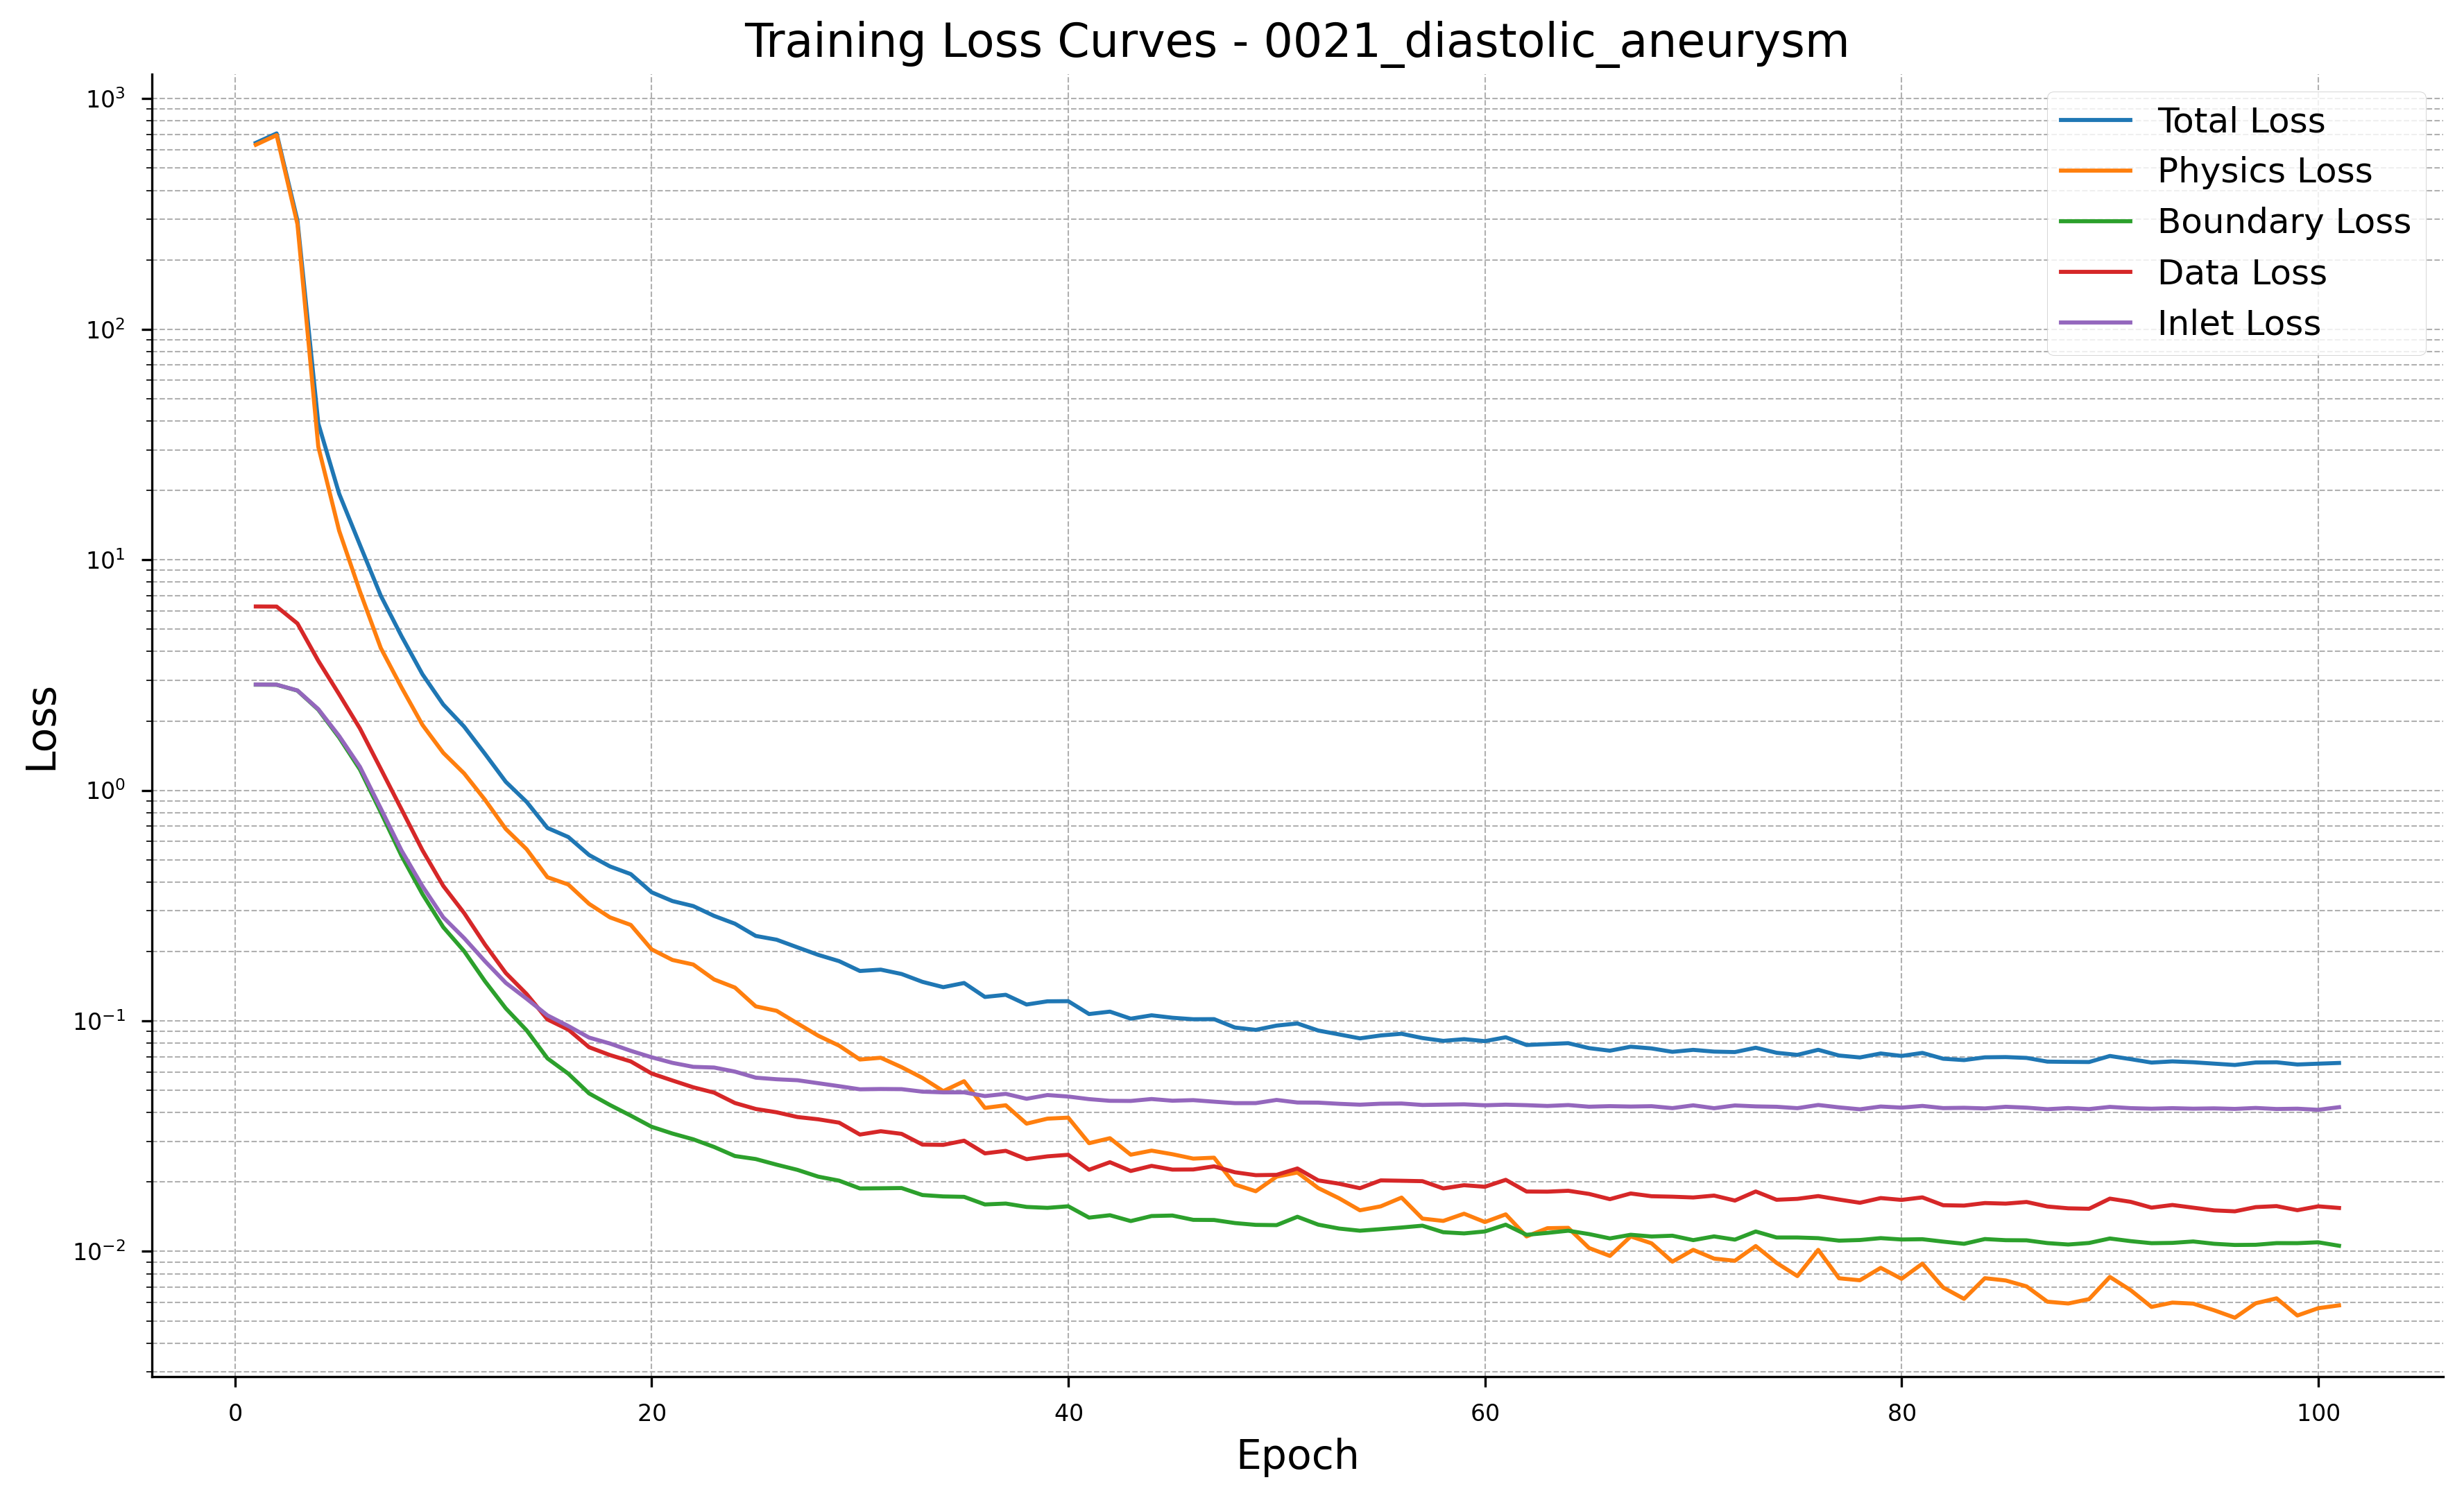
\includegraphics[width=0.9\textwidth]{0021_diastolic_aneurysm/0021_diastolic_aneurysm/loss_curves_0021_diastolic_aneurysm.png}
    \caption{Loss curves for the PINN training process, showing the evolution of the physics, boundary, inlet, and data-fitting losses over 1000 epochs. The self-adaptive loss weighting mechanism effectively balances the contributions of each loss component, ensuring that the network learns realistic flow solutions while adhering to the governing Navier--Stokes equations.}
    \label{fig:loss_curves1}
\end{figure}



\bibliographystyle{unsrtnat}
\bibliography{references}

\end{document}

